
\subsection{Op basis van verstoring door randomisatie}
\label{randomisatie}
\subsubsection{Randomisatie aanpak op basis van Singular Value Decomposition door Polat en Du \cite{Polat:2005:SCF:1066677.1066860}}

Deze werkwijze focust enkel op de privacy van de gebruiker. De gebruiker zal zijn gegevens “vermommen” of eerder verstoren en deze verstoorde data naar de server sturen. De verstoring gebeurt op een manier zodat de server niet de correcte persoonlijke data van de user kent maar eerder de range kent waartussen de waarden liggen. Toch kan de server op deze waarden Collaborative Filtering alsnog uitvoeren. Dit is mogelijk omdat SVD gebaseerd is op geaggregeerde gegevens en niet op individuele waarden.

Men voegt de verstoring toe in drie stappen:
\begin{enumerate}
\item De server beslist welke verdeling men zal gebruiken om de data te verstoren en laat dit de gebruikers weten. Mogelijkheden zijn bijvoorbeeld een uniforme verdeling of een Gaussverdeling.
\item Elke gebruiker berekent Z-scores \footnote{De Z-score of gestandaardiseerde vorm van een stochastische variabele $X$ met verwachtingswaarde $\mu$ en standaardafwijking $\sigma$ is de afwijking van zijn verwachtingswaarde, uitgedrukt in eenheden van de standaardafwijking. In formulevorm:
$Z=\frac{X-\mu}{\sigma}$
De Z-score betekent een gestandaardiseerde waarde die zich met andere Z-scores laat vergelijken.

} voor de waarden van zijn rating vector vult de lege cellen met nullen.
\item De gebruiker genereert per score een randomwaarde op basis van de verdeling aangegeven door de server. Hij voegt deze aan de score toe. Het geheel van de ratings wordt per gebruiker dan doorgestuurd naar de server, deze berekent hiermee de vermomde user-item matrix A’.
\end{enumerate}
\begin{figure}[htpb]   
    \label{Figuur::randomisatiefig}      
  \begin{center}    
 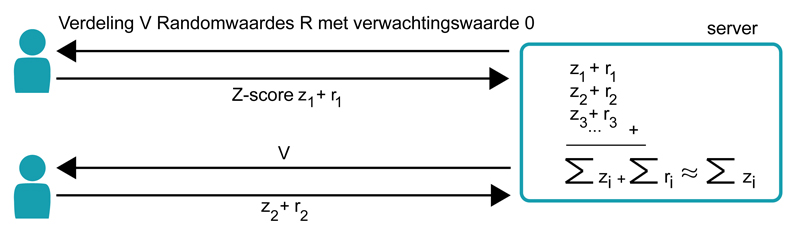
\includegraphics[scale=0.5]{fig/randomisatie}    
  \end{center}   
  \caption{Het basisprincipe bij een oplossing met randomisatie: bij een som over een grote groep gebruikers zal de som over de randomwaardes naar 0 gaan omdat de verwachtingswaarde van hun verdeling 0 is.}  
   \end{figure}
Om aan Singular Value Decomposition te doen heb je een user-feature matrix U en een item-feature matrix V nodig. De item-feature matrix V bereken je op basis van A’\^TA’. De waarden hiervan worden verkregen door het scalair product te nemen van de rijen van de matrix A’\^T en de kolommen van matrix A’. Als men deze som van producten over een groot aantal gebruikers neemt dan zal de waarde van de totale random verstoring naar 0 neigen. Dit komt omdat de random waarde gekozen is uit een verdeling met verwachtingswaarde 0. Uit de eigenwaarden van A’\^TA’. kan men dan de matrix V’ bepalen. De user-feature matrix U’ kan op een gelijkaardige manier benaderd worden met een som over de items. Deze aanpak wordt duidelijk nauwkeuriger naarmate er meer gebruikers en items zijn aangezien de impact van de willekeurig gekozen waarden uit de verdeling meer naar 0 zal neigen bij grotere sommaties.

Hoe meer verstoring, hoe meer privacy de gebruiker heeft maar ook hoe hoger de MAE-waarde en dus hoe slechter de aanbevelingen. Uit tests op de MovieLens en Jester dataset lijkt een keuze van randomwaarden uit de Gaussverdeling met standaarddeviatie 1 de beste resultaten te geven. Bij 100 gebruikers in de MovieLens dataset is de MAE zonder verstoring ongeveer 0.7146 en met verstoring 0.7964. Omdat de MovieLens database met een ratingsysteem werkt van 1 tot 5 sterren geeft het kleine verschil van 0.0818 in de MAE aan dat de kwaliteit van de aanbevelingen niet veel inboet door de aangebrachte verstoring.  De resultaten zijn bij nog meer gebruikers zoals verwacht zelfs nog beter. De Jester dataset gaf gelijkaardige resultaten.\\

Belangrijke kenmerken :
\begin{itemize}
 
\item Berekeningen van de aanbevelingen gebeuren op de server.
\end{itemize}
Voordelen : 
\begin{itemize}
\item Geen berekeningen aan client-zijde.
\end{itemize}
Nadelen:
\begin{itemize}
\item Biedt geen volledige privacy, de provider heeft nog steeds een idee in welke range de ratings liggen afhankelijk van de gebruikte verstoring. 
\item Werkt minder nauwkeurig met kleinere datasets.

\end{itemize}
